\documentclass[UTF8,10pt,titlepage,a4paper]{ctexart}
\usepackage[margin=1in]{geometry}
\usepackage{hyperref}
\hypersetup{hidelinks}
\usepackage{listings}
\usepackage{xcolor}
\usepackage{dirtree}
\usepackage{graphicx}
\usepackage{setspace}
\setlength{\parindent}{2em}
\renewcommand{\baselinestretch}{1.5}
\usepackage{enumitem}
\setitemize[1]{itemsep=-1pt}
\lstset{tabsize=2,
    numbers=left, 
    numberstyle= \tiny, 
    keywordstyle= \color{ blue!70},
    commentstyle= \color{red!50!green!50!blue!50}, 
    frame=shadowbox, % 阴影效果
    rulesepcolor= \color{ red!20!green!20!blue!20} ,
    escapeinside=``, % 英文分号中可写入中文
    xleftmargin=2em,xrightmargin=2em, aboveskip=1em,
    framexleftmargin=2em
}


\title{车牌识别系统}
\author{田阳 \thanks{计算机技术12018002098}}
\date{\today}
\pagestyle{plain}

\begin{document}
\thispagestyle{empty}
\begin{figure}[t]
\vskip 2cm
\begin{center}

\includegraphics[scale=0.6]{ynu.jpg} \\
\end{center}
\end{figure}
\begin{center}
   \quad \\
  {\kaishu \zihao{3} \textbf{《图像处理与计算机视觉》期末作业}}
\end{center}
\vskip 2.5cm
\begin{flushleft}
    \songti \zihao{4}
		\par\setlength\parindent{8em}
    \quad 
    
    专\hspace{0.61cm}业 :\underline{计算机技术\quad}

    年\hspace{0.61cm}级:\underline{\qquad研一\qquad}

    学\hspace{0.61cm}号:\underline{\qquad田阳\qquad}

  	姓\hspace{0.61cm}名:\underline{12018002098\quad}
    \vskip 3cm
    \centering
    2019.7.31
\end{flushleft}


\newpage
\thispagestyle{empty}
\tableofcontents
\newpage
\setcounter{page}{1}
\section{实验要求}
\subsection{项目简介}
本次实验要求实现一个车牌识别系统,车牌识别系统(LPR)较为常见,通常可见于停车站,收费站,门卫系统
等,它利用计算机视觉识别技术对车牌进行预处理,定位,字符分割,字符识别等操作可准确识别出车牌的信
息。
\subsection{主要步骤}
对于图像的识别一般都有以下步骤:
\begin{enumerate}
\item 预处理即是对摄像机拍摄到的包含车牌的图像进行一系列处理,使其能够对接下来的步骤提供良好的图像质量。由于光照因素,
运动因素等外部环境对成像质量造成的影响,可用以下常见的方法消除:
\begin{itemize}
  \item 用逆波法消除匀速运动造成的图像模糊;
  \item 用滤波法,比如中值滤波,均值滤波等消除可见噪点;
  \item 用灰度拉伸及直方图均衡等对图像区域进行强化;
\end{itemize}
\item 车牌定位即对图像区域进行搜寻,找到符合预设的候选区,比如此次实验中的车牌,然后对候选区域
进一步分析,评判,找出最优的候选区。
\item 字符分割即对定位到的区域分割成单个字符,分别进行处理。
\item 字符识别即对分割字符进行字符串化输出,一般可基于神经网络,支持向量机,开放api等方式进行
识别。
\end{enumerate}
\begin{itemize}
  \item[*] \textbf{流程图} \\
  \begin{figure}[h]
    \centering
    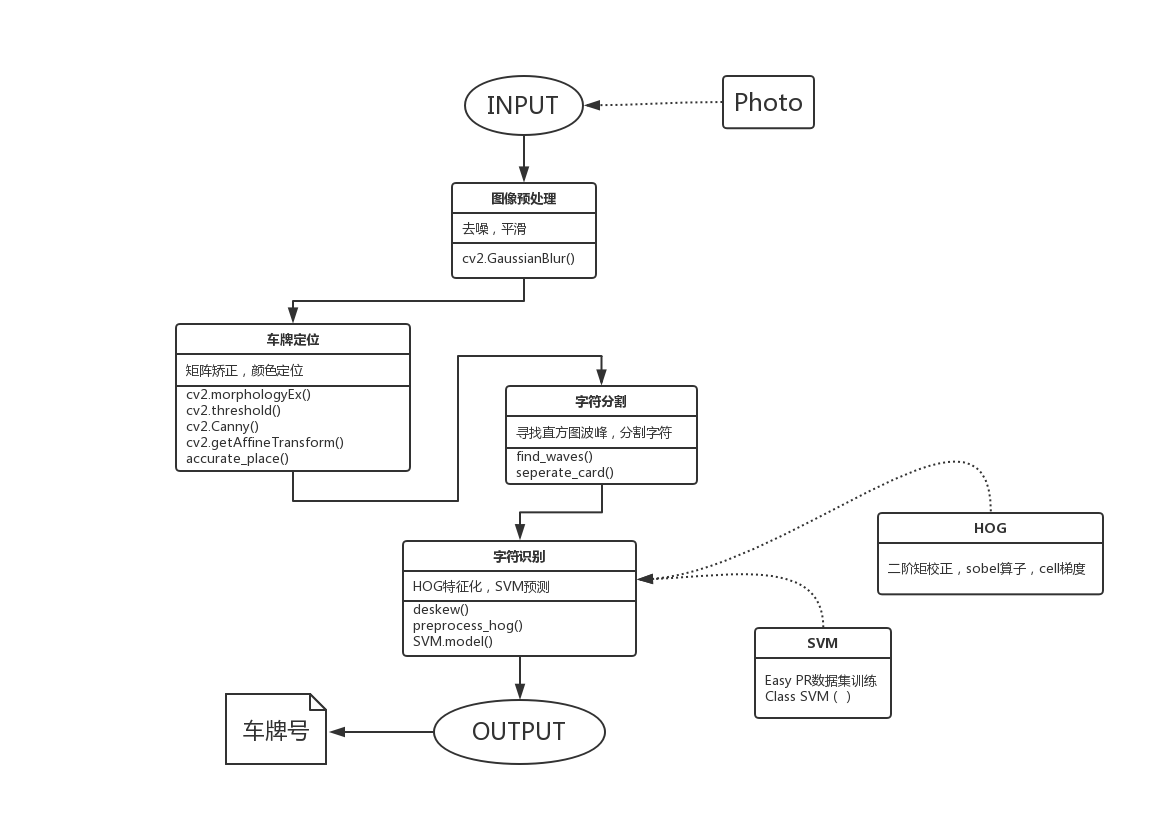
\includegraphics[width=.6\textwidth]{flow.jpg}
    \caption{流程图}
  \end{figure}  
\end{itemize}

\section{实验内容}
\subsection{实验环境}
\begin{itemize}
  \item \textbf{配置}
  \begin{itemize}
    \item[*] \emph{系统:win10 }
    \item[*] \emph{CPU:Intel(R) Core(TM) i5-8400}
    \item[*] \emph{RAM: DDR4 16GB}
    \item[*] \emph{硬盘:1.8T HD}
  \end{itemize}
  \item \textbf{工具}
  \begin{itemize}
    \item[*] \emph{编程工具:VScode}
    \item[*] \emph{python:3.7.4}
    \item[*] \emph{图形界面:tkinter}
    \item[*] \emph{机器学习库:OpenCV}
  \end{itemize} 
\end{itemize}
\subsection{数据准备}
本次实验的训练集来自gitee开源数据集\emph{EasyPR}\footnote{https://gitee.com/easypr/EasyPR},
此数据集专门用于车牌识别。其中包含两类两份文件,分别命名为\emph{chars2.7z}以及
\emph{charsChinese.7z},前者是手写数字[0-9]以及手写字母[A-Z]的集合,后者是部分省简称的手写汉字。
\subsection{项目结构}
\begin{figure}[h]
\dirtree{%
.1 /.
.2 train.
.3 chars2.7z.
.3 charsChinese.7z.
.2 test.
.2 latex.
.2 config.js.
.2 surface.py.
.2 predict.py.
.2 svm.dat.
.2 svmchinese.dat.
}
\caption{Project Tree}
\label{ref:tree}
\end{figure}
图\ref{ref:tree}是本项目的目录结构,\emph{train}以及\emph{test}分别是项目的训练集以及用于测试
的图片,\emph{config.js}则是用于车牌识别的部分参数,\emph{surface.py}以及\emph{predict.py}
分别是车牌识别系统的图形界面及后台核心代码,\emph{dat}后缀的文件则是在训练后保存的模型数据。
\subsection{核心代码}
本项目仍然是按照车牌识别系统的一般步骤进行,即图像预处理,车牌定位,字符分割及字符识别。
\subsubsection{图像预处理}
图像预处理即是对图像进行简单的去噪,转换灰度图等操作。
\begin{lstlisting}[language=python]
blur = self.cfg["blur"]
if blur > 0:
	img = cv2.GaussianBlur(img, (blur, blur), 0)
oldimg = img
img = cv2.cvtColor(img, cv2.COLOR_BGR2GRAY)
\end{lstlisting}
\verb|cv2.GaussianBlur|实现的是高斯模糊,其本质上是低通滤波器,输出图像的每个像素点是原图像上对应像素点
与周围像素点的加权和。高斯滤波的卷积核权重并不相同,中间像素点权重最高,越远离中心的像素权重越小高斯滤波
相比均值滤波效率要慢,但可以有效消除高斯噪声,能保留更多的图像细节。\verb|cvtColor|则是进行图像空间转换,
将彩色图片转换为灰度图,方便下列步骤进行。
\subsubsection{车牌定位}
车牌定位的方法和步骤较多,为了获取较为准确的车牌位置,我按照以下步骤进行:
\begin{enumerate}
  \item \textbf{获取轮廓} \par
  \begin{lstlisting}[language=python]
  kernel = np.ones((20, 20), np.uint8)
	img_opening = cv2.morphologyEx(img, cv2.MORPH_OPEN, kernel)
	img_opening = cv2.addWeighted(img, 1, img_opening, -1, 0)
  ret, img_thresh = cv2.threshold(img_opening, 0, 255,
                cv2.THRESH_BINARY + cv2.THRESH_OTSU)
	img_edge = cv2.Canny(img_thresh, 100, 200)
  \end{lstlisting} 
  上述即是定位轮廓的一般步骤,由于篇幅有限,我只摘取了部分代码用来解释(下同)。此处用到了形态学中的\emph{开闭运算},
  二者的不同只是\emph{膨胀}与\emph{腐蚀}的先后顺序不同,二者目的在于去除图像中的黑点或黑洞,平滑边界,
  以期去除非车牌区域。\emph{阈值化}及\emph{Canny}函数用来进一步显示清晰轮廓。
  \item \textbf{定位候选区域} \par
  在上一步中获取的图像的前提下,进一步用\verb|cv2.findContours|找出矩形区域,此为候选区,车牌
  即在其中,再用之前定义的车牌特征\footnote{长宽比在2到5.5之间,车牌最大面积为2000},来将其余的矩形排除。
  \item \textbf{精确定位\footnote{此处代码在\emph{predict.py}的[306-435]行}}\\
  此处也分两步,矩形矫正(仿射变换)以及利用颜色\footnote{目前只识别蓝绿黄车牌}定位:
  \begin{itemize}
    \item \textbf{矩形矫正}:若将候选车牌命名为\emph{rect},则车牌的角度为\verb|rect[2]|,车牌的坐标可用\verb|cv2.boxpoints|
    取得,则可根据以上特征来进行仿射变换。
    \begin{lstlisting}[language=python]
    M = cv2.getAffineTransform(pts1, pts2)
		dst = cv2.warpAffine(oldimg, M, (pic_width, pic_hight))
    \end{lstlisting} 
    代码块中前者获取新处理后图片与原图片的仿射矩阵,后者进行仿射变换,微调图像的角度。
    \item \textbf{颜色定位}:将灰度图转换为HSV图,获取HSV值,确定候选区域车牌的颜色,然后根据颜色再次定位,
    以期获取更为精确的车牌区域。这里用到自定义函数\verb|accurate_place|,其根据hsv图中获取到的各值来返回车牌坐标。
    \begin{lstlisting}[language=python]
def accurate_place(self, card_img_hsv, limit1, limit2, color):
    ...
    for i in range(row_num):
			count = 0
			for j in range(col_num):
				H = card_img_hsv.item(i, j, 0)
				S = card_img_hsv.item(i, j, 1)
				V = card_img_hsv.item(i, j, 2)
				if limit1 < H <= limit2 and 34 < S and 46 < V:
					count += 1
			if count > col_num_limit:
				if yl > i:
					yl = i
				if yh < i:
          yh = i
    ...
    \end{lstlisting} 
    依次遍历HSV图片,根据获取到的limit值,即车牌颜色范围的上下限,可精确获取到车牌的坐标值。
  \end{itemize}
\end{enumerate}
\subsubsection{车牌分割}
\begin{lstlisting}[language=python]
...
wave_peaks = find_waves(y_threshold, y_histogram)
...
cur_dis = 0
	for i,wave in enumerate(wave_peaks):
		if wave[1] - wave[0] + cur_dis > max_wave_dis * 0.6:
			break
	  else:
			cur_dis += wave[1] - wave[0]
	if i > 0:
		wave = (wave_peaks[0][0], wave_peaks[i][1])
		wave_peaks = wave_peaks[i+1:]
    wave_peaks.insert(0, wave)
...
part_cards = seperate_card(gray_img, wave_peaks)
\end{lstlisting} 
根据预先设定好的函数\verb|find_waves|来分别找到水平及垂直方向的直方图波峰,水平方向的波峰为车牌区域,垂直方向的波峰至少大于
6个,以期分割车牌上的字符。行[4-17]则为在判断波峰是否为左边缘的前提下分离字符。最后根据自定义函数\verb|seperate_card|分割,
返回分割后图片。
\subsubsection{字符识别}
为了能用SVM对图像进行分类,其输入的是描述图像的特征值。一般的方法是HOG+SVM,为介绍这个方法,在此对HOG做出作出解释:
\begin{itemize}
  \item[*] \textbf{HOG}\\
  方向梯度直方图(Histogram of Oriented Gradient, HOG)特征是一种在计算机视觉和图像处理中用来进行物体检测的特征描述子。
  它通过计算和统计图像局部区域的梯度方向直方图来构成特征。在一副图像中,局部目标的表象和形状能够被梯度或边缘的方向密度
  分布很好地描述。HOG实现的方法是首先将图像分成小的连通区域,我们把它叫细胞单元。然后采集细胞单元中各像素点的梯度的或边缘的方向直方图。
  最后把这些直方图组合起来就可以构成特征描述器。
\end{itemize}
具体的代码可见下:
\begin{lstlisting}[language=python]
def deskew(img):
m = cv2.moments(img)
if abs(m['mu02']) < 1e-2:
	return img.copy()
skew = m['mu11']/m['mu02']
M = np.float32([[1, skew, -0.5*SZ*skew], [0, 1, 0]])
img = cv2.warpAffine(img, M,
   (SZ, SZ), flags=cv2.WARP_INVERSE_MAP | cv2.INTER_LINEAR)
return img
\end{lstlisting} 
这段代码是对图像进行二阶矩校正,为下一步做准备。
\newpage
\begin{lstlisting}[language=python]
def preprocess_hog(digits):
samples = []
for img in digits:
	gx = cv2.Sobel(img, cv2.CV_32F, 1, 0)
	gy = cv2.Sobel(img, cv2.CV_32F, 0, 1)
	mag, ang = cv2.cartToPolar(gx, gy)
	bin_n = 16
	bin = np.int32(bin_n*ang/(2*np.pi))
	bin_cells = bin[:10,:10], bin[10:,:10], bin[:10,10:], bin[10:,10:]
	mag_cells = mag[:10,:10], mag[10:,:10], mag[:10,10:], mag[10:,10:]
  hists = [np.bincount(b.ravel(), m.ravel(), bin_n) 
            for b, m in zip(bin_cells, mag_cells)]
	hist = np.hstack(hists)
  # transform to Hellinger kernel
	eps = 1e-7
	hist /= hist.sum() + eps
	hist = np.sqrt(hist)
	hist /= norm(hist) + eps
	samples.append(hist)
	return np.float32(samples)
\end{lstlisting} 
这段代码较为重要,因此我将HOG的函数表达全部摘录于此,以期做详细的介绍。要找到每个单元格的HOG描述符,就要在X和Y方
向上找到每个单元的Sobel导数,然后在每个像素处找到它们的大小和梯度方向,该梯度量化为16个整数值,将此图像分为四个子方块,对于
每个子平方,计算方向的直方图(16个区间),用它们的大小加权,因此每个子方格都会为您提供一个包含16个值的向量,四个这样的
矢量(四个子方块)一起给出了包含64个值的特征向量,这是我们用来训练数据的特征向量。于是便可以用此函数对图像进行处理,送入SVM
进行训练了。\\
之后便可调用SVM类\footnote{openCv自带SVM模型,可直接调用},只需输入相应参数,便可以将进行训练了。
\subsection{图形界面}

\begin{enumerate}
  \item \textbf{主界面}\\
  \begin{figure}[h]
    \centering
    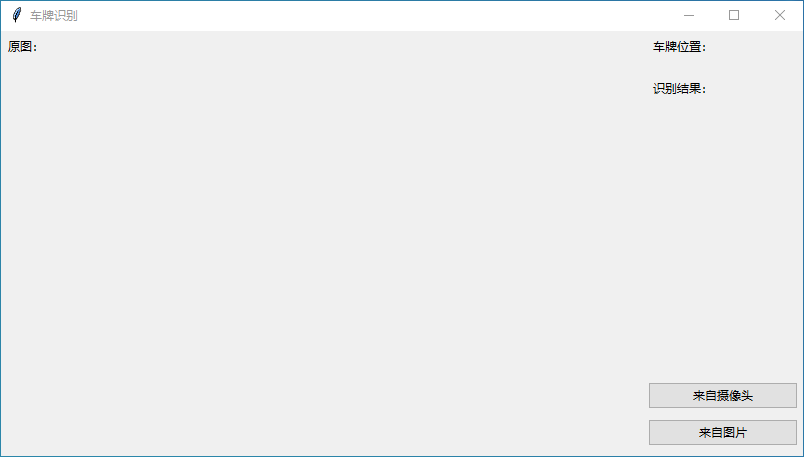
\includegraphics[width=.8\textwidth]{ui.png}
    \caption{主界面}
  \end{figure}\\
为了简化步骤,此项目只是简单的用Tkinter来绘制前端页面,可见此前端可调取两个来源,分别是摄像头
以及本机图片;左边空白处显示选取的图片,右上角返回定位到的车牌区域以及识别结果。
此处只展示界面,代码详情可见文件\emph{surface.py}内。
  \item \textbf{运行界面}\\
  \begin{figure}[h]
    \centering
    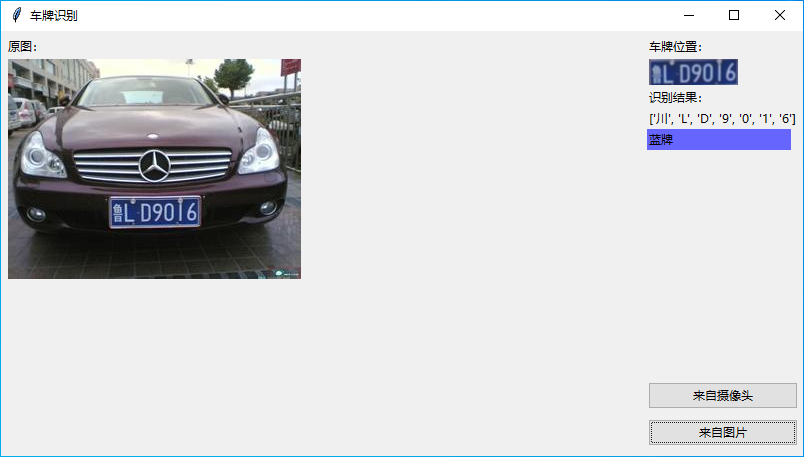
\includegraphics[width=.8\textwidth]{run.png}
    \caption{运行界面}
  \end{figure}\par
当选取了一张图片后,图片会展示在界面左端,右上角展示车牌及其结果,此次只是一次简单的测试,并不适用
于任何图片,其正确与否与图片的质量,光照环境,清晰度,拍摄角度有关,但一般来说能够识别出大部分图片,
但准确率仍有提高的空间。
\end{enumerate}
\newpage
\section{总结}
此次实验是基于github上的项目改造而来\footnote{https://github.com/yinghualuowu},在作者优秀的
代码基础上,我加上了部分我的修改与理解。此项目结合了图像处理及机器学习相关知识,在阅读及修改
代码的过程中,我感到受益匪浅。此项目的图像处理内容基于opencv库,opencv封装了大量图像处理方面的
算法及工具,比如\emph{形态学}方面的\verb|cv2.morphologyEx|及涉及到仿射变换的\verb|cv2.warpAffine|
等函数接口,也基于此我也学习到了直方图,仿射变换,形态学的开闭运算及图像处理中的高斯去噪及阈值化
等诸多知识点,填补了我在此方面的空白。\par
同时,SVM和HOG让我学习到了图像处理及机器学习的结合,HOG是对图像特征的提取,SVM是对图像的分类,
前者提供的特征量是对后者的输入。二者结合,就能准确对车牌信息进行识别。\par
此次实验仍然存在诸多不足:
\begin{itemize}
  \item 少部分图像有无法识别的现象,原因可能出自客观环境,比如图片质量不佳及拍摄角度过大等,也
  可能是算法本身的问题,比如仿射变换算法的不完善,定位算法的不精确等。
  \item 未能通过大量的实验来计算本系统的各方面性能。
\end{itemize}
总的来说,此次实验让我对\emph{图像处理与计算机视觉}这门课程有了更深入的认识。
\newpage
\begin{thebibliography}{99}
    \bibitem{1} \href{https://blog.csdn.net/qq878594585/article/details/81838260}{cv2.warpAffine参数详解}\footnote{可点击文献名直接跳转网址}
    \bibitem{2} \href{https://blog.csdn.net/GDFSG/article/details/51015066}{图像的几何矩}
    \bibitem{3} \href{https://blog.csdn.net/liulina603/article/details/8291093}{目标检测的图像特征提取之(一)HOG特征}
    \bibitem{4} \href{https://zhuanlan.zhihu.com/p/48200186}{opencv实战从0到N (13)—— svm分类器训练}
    \bibitem{5} \href{https://blog.csdn.net/sinat_34604992/article/details/53933004}{Opencv之HOG特征与SVM相结合的人体检测}
    \bibitem{6} \href{https://www.jianshu.com/p/ef67cacf442c}{图像翻转,平移,仿射及透视 warpAffine}
    \bibitem{7} \href{https://blog.csdn.net/qq_24237837/article/details/77850496}{python-opencv 的minAreaRect的详解}
    \bibitem{8} \href{https://www.cnblogs.com/my-love-is-python/p/10397482.html}{canny边缘检测}
    \bibitem{9} \href{https://www.cnblogs.com/yinliang-liang/p/9293310.html}{二值化的cv2.threshold}
    \bibitem{10} \href{https://blog.csdn.net/zh_jessica/article/details/77992578}{Python-OpenCV 图像叠加or图像混合加权实现}
    \bibitem{11} \href{https://blog.csdn.net/sunny2038/article/details/9137759}{OpenCV-Python教程-形态学处理)}
\end{thebibliography}
\end{document}



